
\section{Motivation}

\subsection{Statement of Purpose}
This dissertation will present measurements for, 

\begin{enumerate}
  \item the SIDIS structure function combination $F_{UU,T} + \epsilon F_{UU,L}$, as well as the structure function $F_{UU}^{\cos\phi}$, and $F_{UU}^{\cos(2\phi)}$.  These quantities will be extracted for $\pi^+$ and $\pi^-$ from the differential cross section.
  \item the SIDIS structure function $F_{LU}^{\sin\phi}$.  This will be extracted from beam spin asymmetry measurements for $K^{+}$.
\end{enumerate}

\subsection{Motivation}

%The field of nuclear and particle physics grew tremendously during the middle part of the 20th century.  As the Stanford Linear Accelerator (SLAC) accelerated electrons and collided them into various types of targets, previously unknown particles were discovered rapidly.  The abundance of particles was eventually explained by Gell-Man and Zweig with the inclusion of a set of new fundamental particles called quarks that carried a new degree of freedom known as color.  These ideas birthed the Quark Model which successfully predicted the masses and existence of new particles made of quarks, and eventually grew into Quantum Chromodynamics (QCD).  \\

%A key feature of Quantum Chromodynamics is confinement; bound states of quarks must be colorless and thus quarks cannot be directly observed outside of the hadrons they compose.  During the last 50 years, quark momenta within hadrons has been studied successfully with co-linear parton distribution functions (PDFs).  At leading order these functions $f(x)$ can be interpreted as the probability to find a quark with a co-linear (along the direction of the momentum transfer from the probe) momentum fraction $x$ in a hadron.  However, the one-dimensional momentum distributions don't tell the full story of what's happening inside the hadron, and during the last 15-20 years the focus has shifted to the study of three-dimensional nucleon structure. \\

Transverse momentum dependent parton distribution functions (TMDs) describe quark distributions for a quark with momentum fraction $x$ and a momentum in the transverse plane $\kt$.  TMD functions are expected to be universal, and show up in the cross sections for Drell-Yan ($hh \rightarrow l \bar{l}X$) and semi-inclusive deep inelastic scattering (SIDIS) and other processes.  This thesis work will measure SIDIS.  \\

At leading order (twist two) there are eight TMD functions, each corresponding to different combinations of quark and nucleon spin.  They are shown in figure \ref{fig:tmd-table}.  The Boer-Mulders function $h_{1}^{\perp}$ for example, describes the difference in transverse quark polarization in an unpolarized nucleus.  A non-zero observation of the Boer-Mulders function would imply that quarks have a non-zero orbital angular momentum.  The measurement of $F_{UU}^{\cos\phi}$, and $F_{UU}^{\cos(2\phi)}$ provide data which can be used to test model dependent predictions for the Boer-Mulders function, as well as any future predictions for the structure functions (these need not even be related to the TMD framework).  

\begin{figure}
  \centering
  \includegraphics[width=6cm]{image/TMD-table.jpg}
  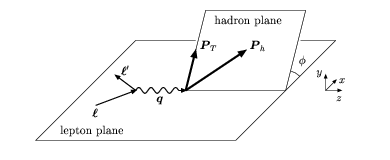
\includegraphics[width=8cm]{image/PhiHadron.png}
  \caption{Left: Leading twist TMD PDFs and their interpretation in terms of different combinations of quark/nucleon spin. Right:  The angle $\phi_h$ shown as the angle between the lepton and hadron planes in a SIDIS event. }
  \label{fig:tmd-table}
 

\end{figure}

Deep Inelastic Scattering (DIS) events are those in which a lepton $e(l)$ collides with a hadron $h(P)$ (in our case a proton), transferring sufficient momentum (sufficiently is an imprecise term, as a working assumption I use $Q^{2} \geq 1.0 \: GeV^{2}/c^{2}$) to the hadron to interact with one of it's constituent partons.  An inclusive event is one in which only the outgoing lepton is identified and the kinematics are calculated based on the difference between the beam leptons and the final state lepton.  Semi-Inclusive DIS (SIDIS) events are those in which one (or more) hadron is detected in the final state along with the scattered lepton $e'(l')$.  

\begin{equation}
  e(l) + h(P) \rightarrow e'(l') + h(P_{h}) + X 
\end{equation}

In SIDIS it is customary to define the following kinematic variables (where $q = l - l'$ and $Q^{2} = -q^{2}$). 

\begin{align}
  x = \frac{Q^{2}}{2P \cdot q} && y = \frac{P \cdot q}{P \cdot l} && z = \frac{P \cdot P_{h}}{P \cdot q} && \gamma = \frac{2Mx}{Q}
\end{align}

Additionally, the ratio $\varepsilon$ of the longitudinal and transverse photon flux is shown below.

\begin{equation}
	\varepsilon = \frac{1 - y - \frac{1}{4}\gamma^2 y^2}{1 - y + \frac{1}{2}y^2 + \frac{1}{4}\gamma^2 y^2}
\end{equation}

The differential cross section for the SIDIS reaction $ep \rightarrow ehX$ can be written in a model independent way using a set of structure functions $F$ \cite{tmds-mulders:1995}.  The differential cross section, without terms due to polarized targets that are not relevant for this thesis, is given below.

\begin{eqnarray}
  \frac{d\sigma^{e^-P\to e^-hX}}{dx_B \, dQ^{2}\, dz\, d\phi_h\, d p_{h\perp}^2} = \frac{\alpha^2_{em}}{2x_B y Q^2} \frac{y^2}{1-\varepsilon}  ( 1+\frac{\gamma^2}{2x_B} ) \Bigl\{ F_{UU ,T} +  \varepsilon F_{UU ,L} \nonumber \\
  + \sqrt{2\,\varepsilon (1+\varepsilon)} \cos\phi_h F_{UU}^{\cos\phi_h}+ \varepsilon \cos(2\phi_h) F_{UU}^{\cos 2\phi_h} +& \lambda_e
\sqrt{2\,\varepsilon (1-\varepsilon)} \sin\phi_h F_{LU}^{\sin\phi_h} \Bigr\}
\end{eqnarray}

Here $\lambda_e$ refers to the helicity of the incoming lepton (beam electron in our case).  If one decomposes the hadronic matrix element which is present in the hadronic tensor into different possible Dirac structures, a set of functions known as transverse momentum dependent parton distributions functions (TMD PDFs) and transverse momentum dependent fragmentation functions (TMD FFs) can be defined.  The structure functions from above can then be calculated as a convolution of these more basic non-perturbative functions.  The notation $\mathcal{C}$ is shorhtand  presented in \cite{tmds-bacchetta:2006} as a way to write structure functions in terms of the convolutions of PDF and FF objects.

\begin{equation}
  \mathcal{C}[\omega f D] = x \sum_{a} e^{2}_{a} \int d^{2}\pt d^{2}\kt \delta^{(2)} \left( z\kt + \pt - \vect{P}_{h\perp} \right) \omega (\kt, \pt) f^{a}(x, k_{T}^{2}) D^{a}(z, p_{T}^{2}) 
\end{equation}

where a is summed over quarks and anti-quarks.  The five structure functions appearing in the cross section are, 

\begin{equation}
F_{UU,T} = \mathcal{C}[f_1 D_1] = x \sum_{a} e^{2}_{a} \int d^{2} \pt d^{2} \kt \delta^{(2)} \left( z\kt + \pt - \vect{P}_{h\perp} \right) f_{1}^{a}(x, k_{T}^{2}) D_{1}^{a}(z, p_{T}^{2})
\end{equation}

\begin{equation}
F_{UU,L} = 0
\end{equation}

\begin{equation}
F_{UU}^{\cos \phi_h} = \frac{2M}{Q} \mathcal{C}[ - \frac{\hhat \cdot \kt}{M_h} \Bigl( x h H_{1}^{\perp} + \frac{M_h}{M} f_1 \frac{\tilde{D}^{\perp}}{z} \Bigr) - \frac{\hhat \cdot \pt}{M} \Bigl( x f^{\perp} D_1 + \frac{M_h}{M} h_1^{\perp} \frac{\tilde{H}}{z} \Bigr)]
\end{equation}

\begin{equation}
F_{UU}^{\cos 2\phi_h} = \mathcal{C}[- \frac{2 (\vect{\hat{h}} \cdot \kt) (\vect{\hat{h}} \cdot \pt) - \kt \cdot \pt}{M M_h} h_{1}^{\perp} H_{1}^{\perp} ]
\end{equation}

\begin{equation}
  F_{LU}^{\sin\phi} = \frac{2M}{Q} \mathcal{C} \Bigl[ -\frac{\hhat \cdot \kt}{M_h} \Bigl( xeH_1^\perp + \frac{M_h}{M} f_1 \frac{\tilde{G}^\perp}{z} \Bigr) + \frac{\hhat \cdot \pt}{M} \Bigl( xg^\perp D_1 + \frac{M_h}{M} h_{1}^{\perp} \frac{\tilde{E}}{z} \Bigr) \Bigr]
\end{equation}

where the previously mentioned Boer-Mulders function $h_{1}^{\perp}$ appears at leading order in the $F_{UU}^{\cos 2\phi_h}$ term.  This dissertation will present measurements of combinations of these 5 structure functions.  The unpolarized terms which carry $UU$ indices will be accessed directly through the SIDIS cross section, and the $F_{LU}^{\sin\phi_h}$ term will be measured by measuring the beam spin asymmetry.  The beam spin asymmetry (BSA) is defined as the cross section difference (with respect to the 2 beam helicity states) over the total cross section.

\begin{equation}
  BSA = \frac{d\sigma^+ - d\sigma^-}{d\sigma^+ + d\sigma^-} = \frac{\phimod{LU}{\sin\phi}}{1 + \phimod{UU}{\cos\phi} + \phimod{UU}{\cos(2\phi)}}
\end{equation}

Where the coefficient $A_{LU}^{\sin\phi}$ is defined as, 

\begin{equation}
  A_{LU}^{\sin\phi} = \sqrt{2\,\varepsilon (1-\varepsilon)} \frac{F_{LU}^{\sin\phi}}{F_{UU,T} + \varepsilon F_{UU,L}}
\end{equation}

This asymmetry is particularly interesting because all of the terms that appear in the expansion of the structure function have a pure twist-3 contribution.  If the measurement of this BSA is therefore non-zero, it indicates a sizable contribution of twist-3 TMD functions.  This effect has been observed to be non-zero previously for $\pi$ mesons in the work of \cite{tmds-gohn:2014}.  

